% Standalone supplementary material. Compile with pdflatex.
\documentclass[12pt,a4paper]{article}
\usepackage[margin=1in]{geometry}
\usepackage{newtxtext,newtxmath}
\usepackage{setspace}
\usepackage{graphicx}
\usepackage{booktabs}
\usepackage{caption}
\usepackage{longtable}
\usepackage[hidelinks]{hyperref}
\onehalfspacing
\captionsetup{font=small,labelfont=bf,justification=raggedright,singlelinecheck=false}
\renewcommand{\thetable}{S\arabic{table}}
\renewcommand{\thefigure}{S\arabic{figure}}
\graphicspath{{./}}

\begin{document}

\begin{center}
{\Large\bfseries Supplementary Material}\\[8pt]
{\itshape Treatment Limitation Documentation and Risk Adjusted Mortality
Benchmarking in 190 US Intensive Care Units}\\[6pt]
Fabrice T. Nyambod, MD, MPH
\end{center}

\vspace{10pt}
\noindent\textbf{Contents}

\begin{itemize}\setlength{\itemsep}{0pt}
\item Table S1. Discrimination and accuracy on held out data
\item Table S2. Effect of modeling treatment limitation on unit ranking
\item Table S3. Unit level case mix and limitation rate, provided as a data file
\item Table S4. Unit level ranking comparison, provided as a data file
\item Table S5. Covariate balance before and after weighting, provided as a data file
\item Figure S1. Derivation of the study cohort
\end{itemize}

\newpage

\begin{table}[htbp]
\centering
\small
\caption{Discrimination and accuracy on held out data.}
\label{tab:discrim}
\begin{tabular}{lrrr}
\toprule
Model & AUC & 95\% CI & Brier score \\
\midrule
APACHE IVa                       & 0.8657 & 0.8597 to 0.8717 & 0.0621 \\
APACHE IVa recalibrated          & 0.8657 & 0.8597 to 0.8717 & 0.0605 \\
Plus malignancy                  & 0.8658 & 0.8599 to 0.8718 & 0.0605 \\
Plus limitation status           & 0.8760 & 0.8701 to 0.8818 & 0.0579 \\
Plus limitation and malignancy   & 0.8761 & 0.8702 to 0.8819 & 0.0579 \\
\bottomrule
\end{tabular}

\vspace{2pt}
\footnotesize Held out sample n = 40{,}871. AUC denotes area under the receiver
operating characteristic curve. Adding limitation status improved the AUC
($p<0.001$, DeLong). Adding malignancy did not ($p=0.16$).
\end{table}

\begin{table}[htbp]
\centering
\small
\caption{Effect of modeling treatment limitation on unit ranking.}
\label{tab:rank}
\begin{tabular}{lr}
\toprule
Measure & Value \\
\midrule
Spearman correlation of ranks              & 0.949 \\
Median absolute rank shift                 & 7.5 of 162 \\
Units moving more than 10 positions        & 62 (38.3\%) \\
Units moving more than 20 positions        & 24 (14.8\%) \\
Units changing quartile                    & 38 (23.5\%) \\
Units changing outlier classification      & 13 (8.0\%) \\
\quad High mortality outlier to as expected & 4 \\
\quad As expected to high mortality outlier & 3 \\
\bottomrule
\end{tabular}

\vspace{2pt}
\footnotesize Based on 162 units with 100 or more admissions. Outlier status from
exact Poisson 95\% limits.
\end{table}

\newpage

\begin{figure}[htbp]
\centering
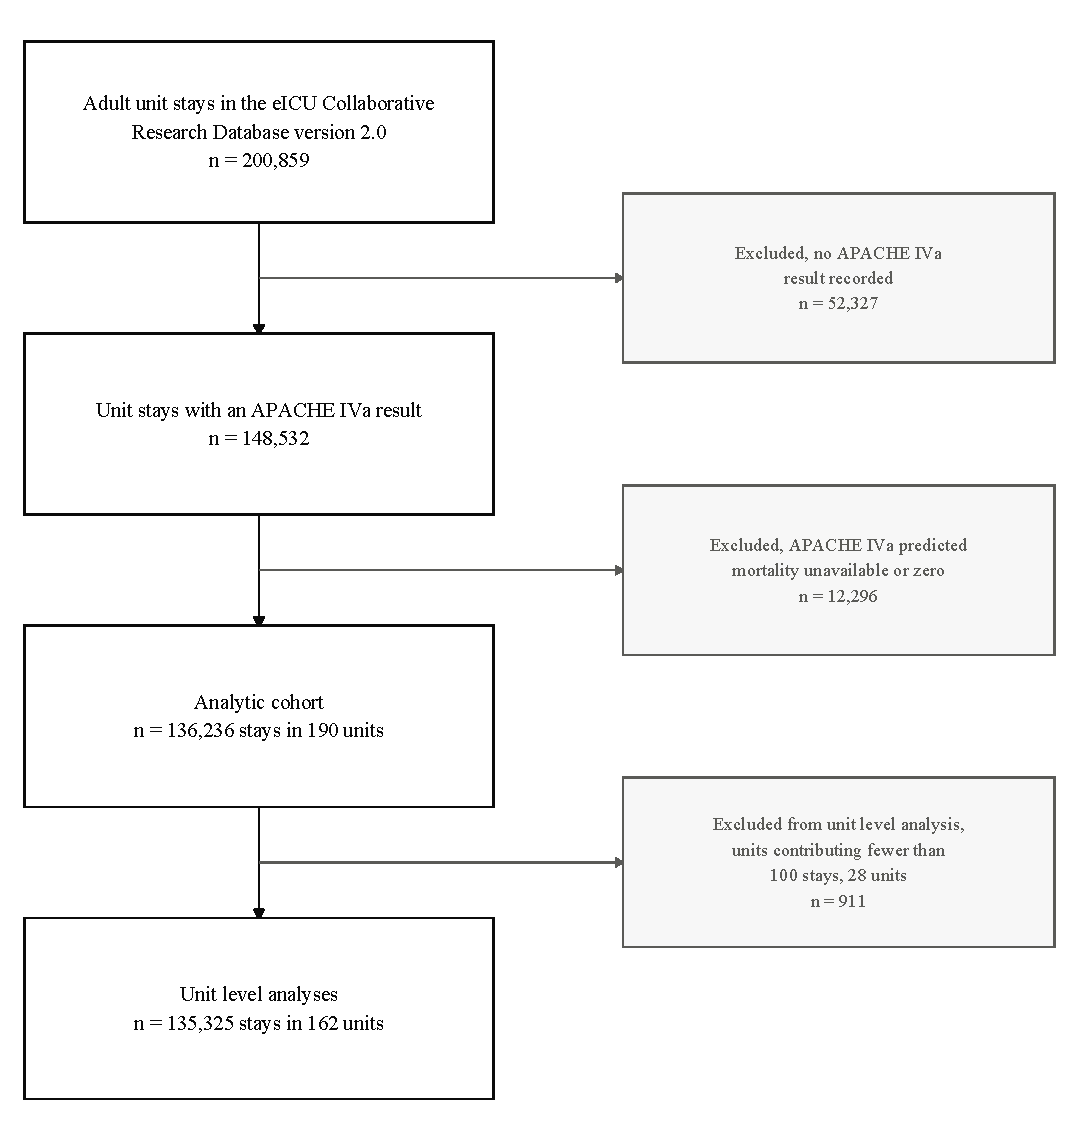
\includegraphics[width=0.42\textwidth]{figures_pdf/FigureS1_flow.pdf}
\caption{Derivation of the study cohort from the eICU Collaborative Research
Database version 2.0.}
\label{fig:flow}
\end{figure}

\vfill
\noindent\footnotesize Tables S3 to S5 accompany this document as
separate data files. They contain unit level aggregates only and no patient
level information.

\end{document}
